\documentclass[twoside, letterpaper, 12pt]{report}
\usepackage{orthodoxservicebook}

\title{The Sunday Reader's Service of the \\ \textsc{Typica} \\  2020 March 22}
\titlepic{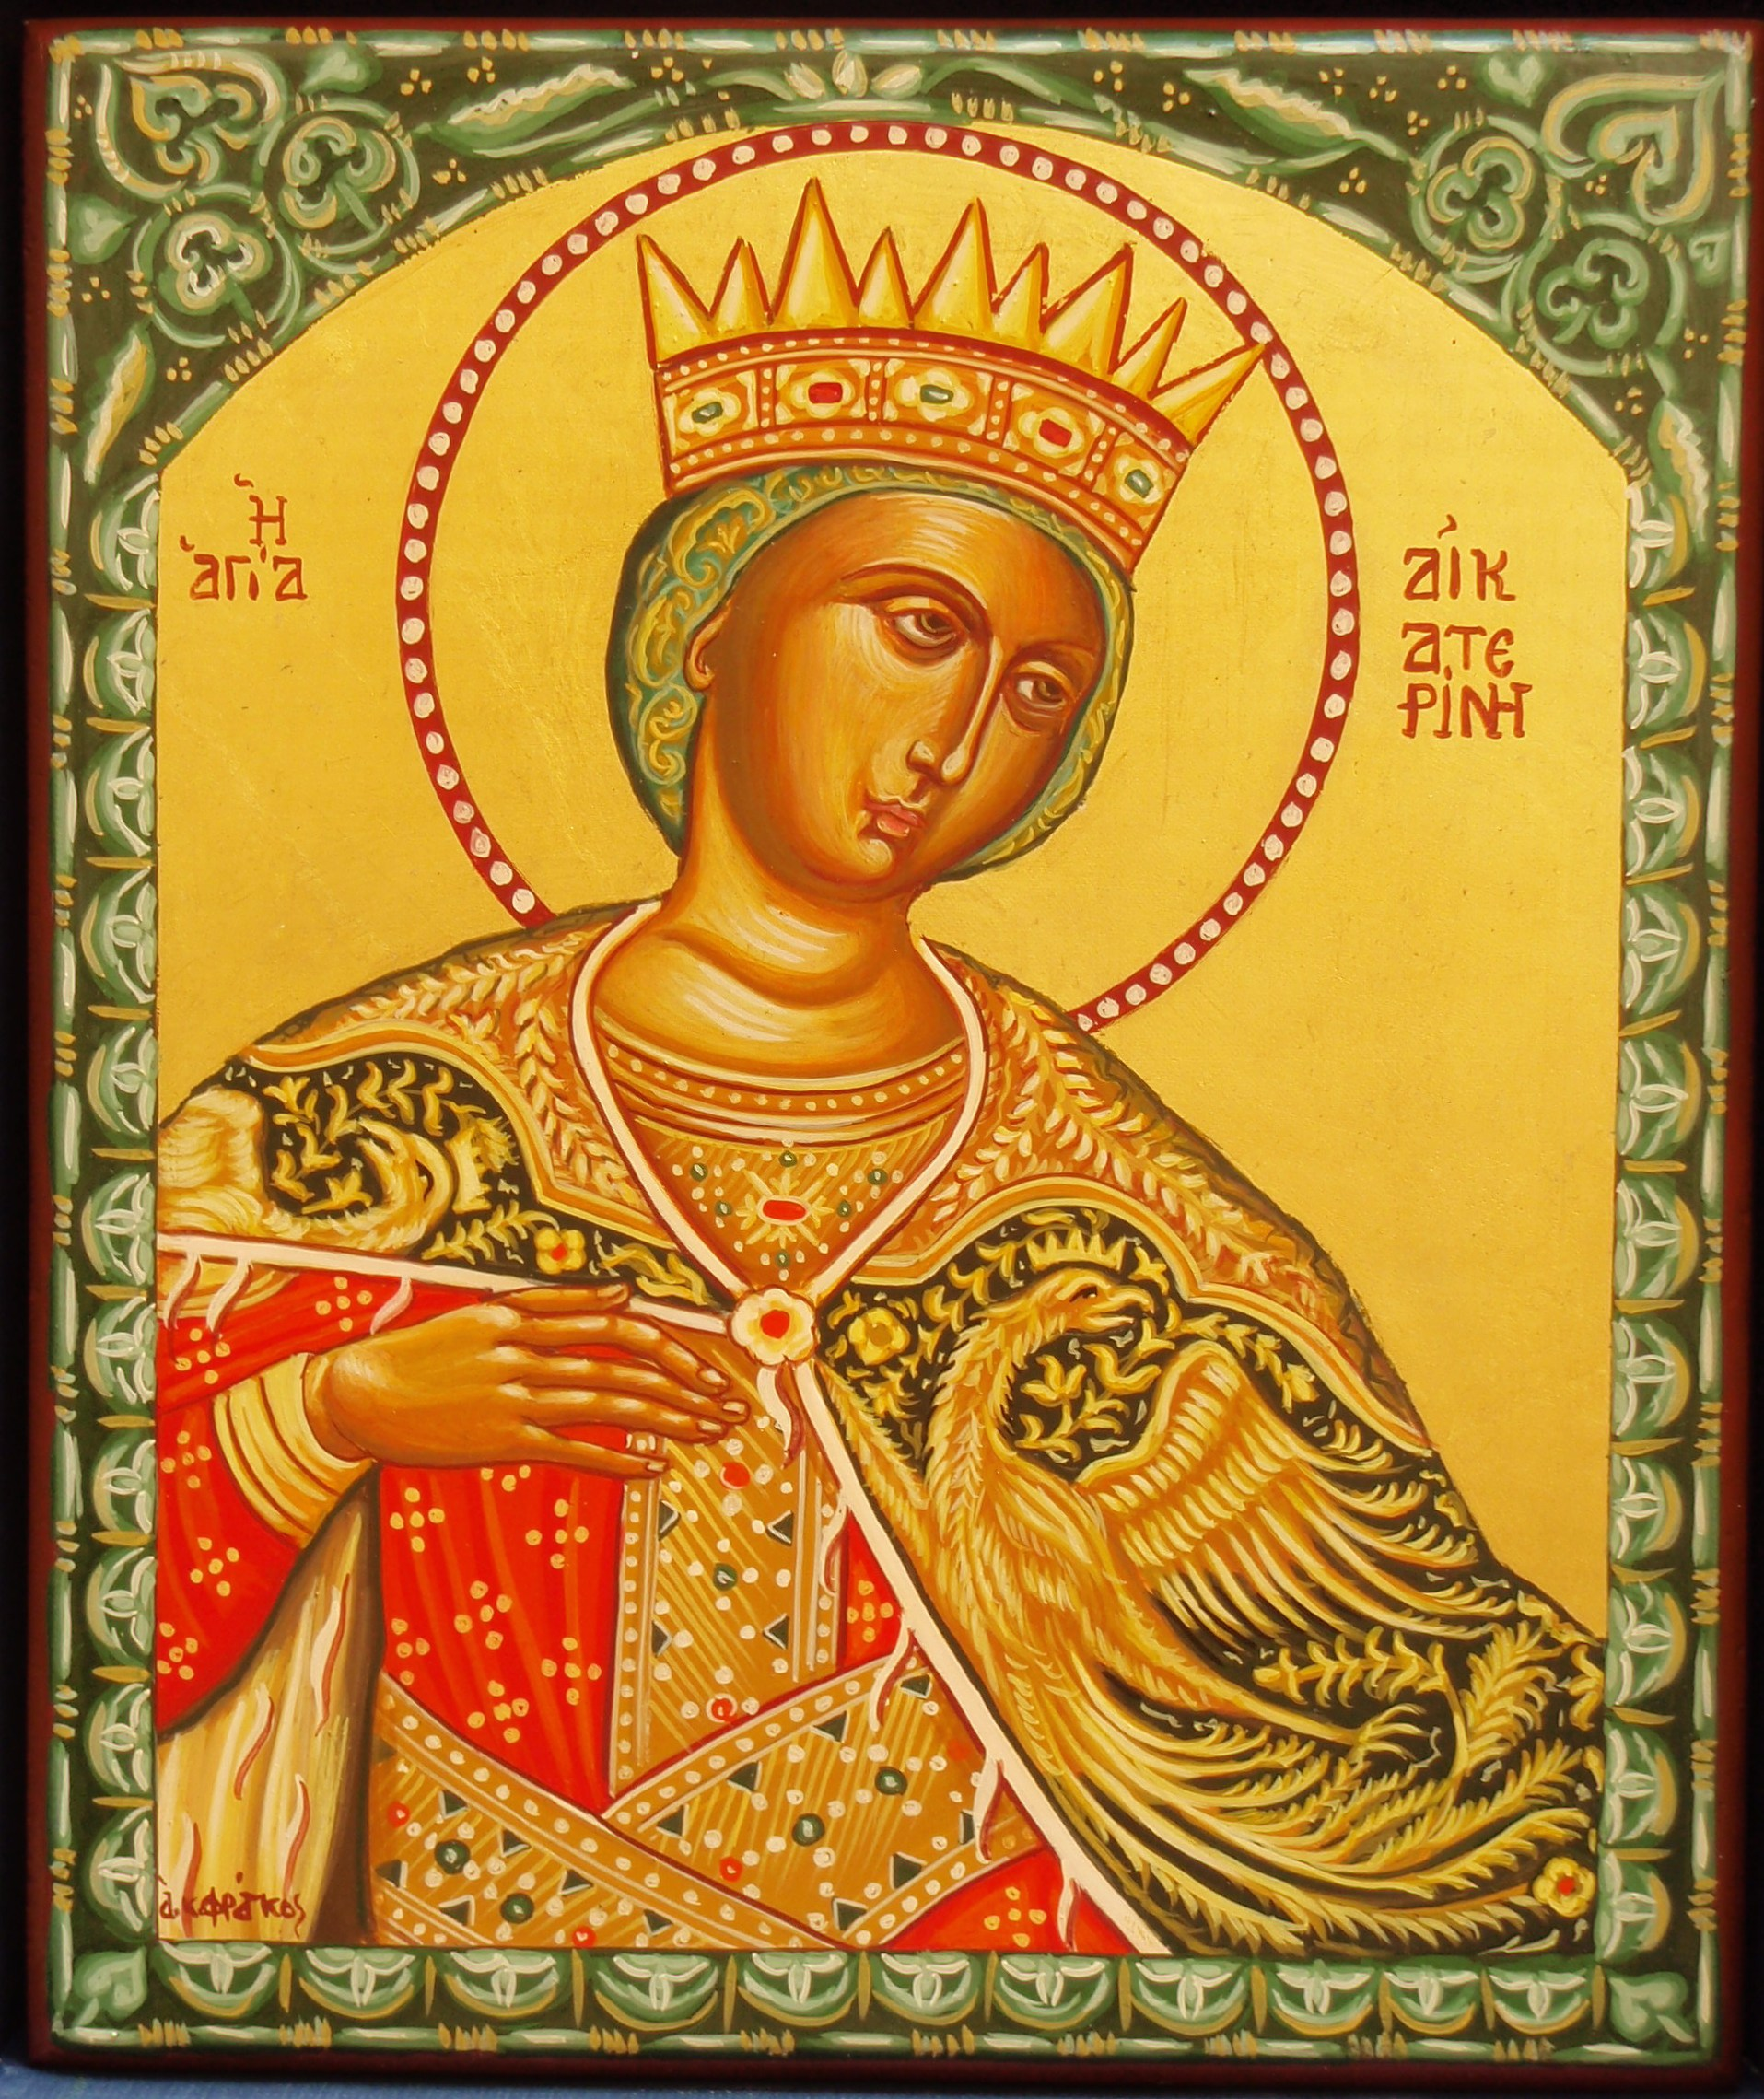
\includegraphics[width=0.5\textwidth]{Katherine1.jpg}}
\date{}
\author{}

\begin{document}
\maketitle
\pagestyle{empty} % Don't show page numbers
\instruction{This page intentionally left blank}
\cleardoublepage
\pagestyle{plain}
\setcounter{page}{1} % Set the page counter to 1 on the first real page
\chapter*{The Sunday Reader's Service of Typica\\ 2020 March 22}
\readerline{Through the prayers of our holy fathers, Lord Jesus Christ our God,
  have mercy on us, and save us}
\lilypondfile{./Z-Responses/Obikhod/Amen.ly}

\trisagionNeedsAmen
\lilypondfile{./Z-Responses/Obikhod/Amen.ly}


\centeredsection{The First Antiphon}
\lilypondfile{./Liturgy/B-FirstAntiphon/BlessTheLord_Greek-Music.ly}

\centeredsection{The Second Antiphon}
\lilypondfile{./Liturgy/C-SecondAntiphon/PraiseTheLord_Greek-Music.ly}

\centeredsection{The Third Antiphon}
\lilypondfile{./Liturgy/D-ThirdAntiphon/Beatitudes_Moscow-Music.ly}

\centeredsection{The Epistle}

\instruction{Both of the New Testament lessons are read
without liturgical introduction or conclusion.
The readers start with “The Reading from…” and proceeds}

\paragraph{The Reading from the Epistle of St. Paul to the Hebrews. (4:14-5:6)}\mbox{}\\

Brethren, since we have a High Priest, Who has passed through the heavens, Jesus, the Son
of God, let us hold fast our confession. For we have not a high priest who is unable to sympathize
with our weaknesses, but One Who in every respect has been tempted as we are, yet without sin.
Let us then with confidence draw near to the throne of grace, that we may receive mercy and find
grace to help in time of need. For every high priest chosen from among men is appointed to act on
behalf of men in relation to God, to offer gifts and sacrifices for sins. He can deal gently with the
ignorant and wayward, since he himself is beset with weakness. Because of this he is bound to
offer sacrifice for his own sins as well as for those of the people. And one does not take the honor
upon himself, but he is called by God, just as Aaron was. So also Christ did not exalt Himself to
be made a high priest, but was appointed by Him Who said to Him, “Thou art My Son, today I
have begotten Thee”; as He says also in another place, “Thou art a priest forever, after the order
of Melchizedek.”

\centeredsection{The Gospel}

\instruction{Both of the New Testament lessons are read
without liturgical introduction or conclusion.
The readers start with “The Reading from…” and proceeds}

\paragraph{The Reading from the Holy Gospel according to St. Mark. (8:34-9:1)}\mbox{}\\

The Lord said, “If any man would come after Me, let him deny himself and take up his
cross and follow Me. For whoever would save his life will lose it; and whoever loses his life for
My sake and the Gospel’s will save it. For what does it profit a man, to gain the whole world and
forfeit his soul? For what can a man give in return for his soul? For whoever is ashamed of Me
and My words in this adulterous and sinful generation, of him will the Son of man also be ashamed,
when He comes in the glory of His Father with the holy angels.” And Jesus said to them, “Truly,
I say to you, there are some standing here who will not taste death before they see the Kingdom of
God come with power.”


\centeredsection{Troparia Before the Creed}
\instruction{Plain reading}
\begin{reader}
\item[Reader 1:] The heavenly choir singeth thy praises, saying:
  Holy, holy, holy, Lord of Sabaoth; heaven and earth are full of Thy glory.

\item[Reader 2:] \emph{Come unto him, and be enlightened,
               and your faces shall not be ashamed.}
  The heavenly choir singeth thy praises, saying:
  Holy, holy, holy, Lord of Sabaoth; heaven and earth are full of Thy glory.

\item[Reader 1:] \emph{\glory}
  The choir of the holy angels and archangels,
  with all the powers of heaven, singeth thy praises, saying:
  Holy, holy, holy, Lord of Sabaoth; heaven and earth are full of Thy glory.

\item[Reader 2:]\emph{\nowandever}
\end{reader}

\centeredsection{The Creed}
\input{Common/TheCreed.txt}


\centeredsection{Prayer of Forgiveness}
\readerline{Forgive, remit, pardon, O God, our sins,
  both voluntary and involuntary, in deed and in word, in knowledge or in ignorance,
  committed by night or by day, in mind and in thought.
  Forgive us them all, for thou art good and lovest mankind.
}


\centeredsection{The Lord’s Prayer}
\input{Common/LordsPrayer.txt}

\readerline{Through the prayers of our holy fathers, Lord Jesus Christ our God, have mercy on us.}
\lilypondfile{./Z-Responses/Obikhod/Amen.ly}


\centeredsection{Kontakia for Sundays in Great Lent}
\lilypondfile{./Menaion/03-25-AnnunciationOfTheTheotokos/AnnunciationOfTheTheotokos-Kontakion-T8-Essey-Music.ly}


\readerline{\lhmForty}

\readerline{
  O Christ our God, Who art worshipped and glorified at all times at every hour both in
  heaven and on earth; Who art long-suffering and plenteous in mercy and compassion; Who lovest
  the just man and showest mercy upon the sinner; and Who callest all men to repentance through 
  the promise of blessings to come; receive, O Lord, at this very hour our supplications, and direct
  our lives in the way of Thy commandments: sanctify our souls, purify our bodies, set our minds
  aright, cleanse our thoughts; deliver us from all affliction, trouble, and distress; compass us about
  with Thy holy angels, that, guided and guarded by them, we may attain unto the unity of the Faith,
  and to the knowledge of Thine unapproachable glory; for Thou art blessed unto ages of ages. Amen.
}

\begin{reader}
  \item \lhmThree{}\\\emph{\gne{}}
  \item \morehonorablethanthetherubim{}
  \item \throughtheprayers{}
\end{reader}

\begin{maybetwocolumns}
\lilypondfile{./Z-Responses/Obikhod/Amen.ly}

\readerline{\blessedbethename{}\thrice{}}

\centeredsection{Psalm 33}
\input{./Psalms/Psalm033-unknowntrans.txt}

\centeredsection{Psalm 144}
\input{./Psalms/Psalm144-unknowntrans.txt}
\end{maybetwocolumns}

\peopleline{\gne}


\centeredsection{A Homily}
\begin{maybetwocolumns}
\instruction{Killing the Fear of Death: Homily for the Third Sunday of Lent
(Adoration of the Cross) Fr. Philip LeMasters, pastor,
St. Luke Antiochian Orthodox Church of Abilene, Texas}

Today we do something that goes against the strongest inclinations of fallen humanity:
We adore and celebrate the Cross. Absolutely no one rejoiced about crosses in the first century,
for crucifixion was the most horrible form of execution the Romans could devise. When the Lord
told Peter plainly that He would be killed, the head disciple was horrified and tried to correct Him.
That is when Christ said to Peter, “Get behind me, Satan, for you are not mindful of the things of
God, but the things of men.” In order words, Peter was thinking like any other human being
enslaved to the fear of death.\\\mbox{}\\

That, of course, is precisely why Jesus Christ offered Himself on the Cross: to set us free from
captivity to the grave. He did not breathe life into us so that we would disappear into the earth,
but so that we would be united eternally with Him in holiness. If we believe our fate is simply for
the decay of the tomb, we will go to great lengths to distract ourselves from the pointlessness of
our existence. So we end up worshiping power, pleasure, possessions, and anything else that staves
off the dread of death. We will make this world a false god in one way or another in a failed effort
to save ourselves on our own terms.\\\mbox{}\\

Today we adore the Cross because through it our Lord has conquered death, making even the tomb
and Hades pathways to the eternal life of the Kingdom through His glorious resurrection. It is
because of His great Self-offering as our High Priest that we may depart this life with the hope of
resurrection and life eternal. But in order to share in the glory of the empty tomb, we must first
follow Him to the Cross by taking up our own crosses. That means dying to the corrupting power
of sin in our lives as we crucify the addiction to self-centered desire that arises from the fear of
death. For if we seek to save our lives by the standards of our fallen world, we will end up losing
our souls.\\\mbox{}\\

Fortunately, there is still time to live as those who are not ashamed of the Cross. We have the
remaining weeks of Lent to prepare to enter into the deep mystery of the Lord Who caused death
to die. And we do not have to look hard for opportunities to do so. They are all around us. For
example, we should turn our attention away from our favorite distractions (e.g. cell phones, video
games, social media, news, sports, and movies) and toward the Lord in daily focused prayer, Bible
reading, and studying the lives and teachings of the Saints. We should sacrifice a small part of our
usual routine by attending Lenten services each week. If our physical health and life circumstances
allow, we should fast as best we can according to the guidelines of the Church. If we cannot fast
from food due to illness, we should learn to accept our struggles with patience, perhaps finding
another area of life where we can practice self-denial. We should give generously of our resources,
time, and attention to others, especially the poor, sick, and lonely. We should serve our family
members, friends, and fellow parishioners instead of simply ourselves. We should pray for our
enemies and do what we can to heal broken relationships. We should stay on guard against
anything that inflames our passions. We should shut out our dark and tempting thoughts with the
Jesus Prayer. We should confess our sins honestly this Lent, and be vigilant against sliding back
into unholy habits.\\\mbox{}\\

It is through such everyday acts of faithfulness that we will take up our crosses and follow the
Savior Who offered Himself on the Cross for our salvation. That is how we will be set free from
the fear of death and all its corrupting effects on our souls. That is how we will adore and celebrate
the Cross as the great sign of our hope, as the only true answer to the tragic brokenness of our
humanity. The God-Man offered Himself on it in order to save us. Now we must offer ourselves
to Him in humble repentance by dying to sin in order to open ourselves to the glory of His
resurrection. That is the Lord’s calling to each and every one of us for, through the Cross, He has
filled all things with joy.

\end{maybetwocolumns}

\centeredsection{Resurrectional Apolytikion in Tone 7}
\lilypondfile{./Octoechos/ResurrectionalApolytikion-Tone7-Kazan-Music.ly}

\centeredsection{Apolytikion for the Holy Cross in Tone 1}
\lilypondfile{./Menaion/09-14-ElevationOfTheCross/ElevationOfTheCross-Tone1ByzChant-Music.ly}

\readerline{\throughtheprayers}

\lilypondfile{./Z-Responses/Obikhod/Amen.ly}

\end{document}

